\section{Regression}

The concepts discussed in the following section could also be presented in
random variables instead of sample ones. As the geometry of sample variables
is almost of no difference comparing to the random ones, the logic of
all the theorems is also the same.


\subsection{Geometry of sample variables}

\marginnote{
\begin{multline*}
\sCorr(x,y) = \frac{\sCov(x,y)}{\sqrt{\sVar(x)\sVar(y)}} \\
= \frac{\frac{1}{n-1}\sum_{i=1}^n (x_i - \bar x)(y_i - \bar y)}
{\sqrt{\frac{1}{n-1} \sum_{i=1}^n (x_i - \bar x)\frac{1}{n-1} \sum_{i=1}^n ( y_i -  \hat y)}}
\end{multline*}
}

In the~same manner it was done in the previous section, we define
the~scalar product of two sample variables
$x =
\begin{pmatrix}
x_1 \\
\vdots \\
x_n
\end{pmatrix}$
and
$y =
\begin{pmatrix}
y_1 \\
\vdots \\
y_n
\end{pmatrix}$
as a sample covariation between them:
\[
\langle x, y \rangle = \sCov(x, y).
\]
The main characteristics of a~vector are its length and direction.
Again, we introduce the~length
\[
\sqrt{\sCov(x,x)} = \sqrt{\sVar(x)} = \sigma_x
\]
and the~angle between two sample variables
\[
\cos(x,y) = \frac{\sCov(x,y)}{\sqrt{\sVar(x)\sVar(y)}} = \sCorr(x,y).
\]
Note that from the definition of the angle
it follows that the~sample correlation coefficient can range from $-1$ to $1$.

\begin{marginfigure}
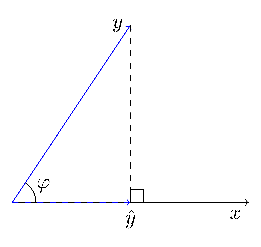
\includegraphics[scale=0.85]{figures/02_basic_projection.pdf}
\caption{Vector $y$ projected onto vector $x$.}
\label{fig:corr_proj}
\end{marginfigure}

Completely analogus to the~case of random variables,
the projection of such a sample variable $y$ onto
$\{cx| c \in \mathbb{R}\}$ is $\hat y = \sCorr(x,y) \cdot y$.

Looking at Figure~\ref{fig:corr_proj}, we can interpret the~square of sample correlation coefficient.
Using the fact that $cos^2 \varphi$ is the~squared ratio of
the~leg adjacent to $\varphi$ to hypotenuse, we can conclude that
\[
\sCorr^2(x,y) = \frac{\sVar(\hat y)}{\sVar(y)},
\]
as the variance of a vector is associated with the square of its length.
Thus, the~sample correlation coefficient squared shows
the~fraction of variance in $y$ which can be explained
with the~most similar vector proportional to $x$.


\subsection{Sample correlation when a constatnt vector added}

\marginnote{
\begin{align*}
\sCorr(x + \alpha \mathbf{1}, y) &= \frac{\sCov(x + \alpha \mathbf{1}, y)}{\sqrt{\sVar(x + \alpha \mathbf{1}) \sVar(y)}} \\
&= \frac{\sCov(x,y) + \sCov(\alpha \mathbf{1},y)}{\sqrt{\sVar(x)\sVar(y)}} \\
&= \frac{\sCov(x,y)}{\sqrt{\sVar(x)\sVar(y)}} \\
&= \sCorr(x,y)
\end{align*}
}

\begin{theorem}
Adding a~vector of constants does not affect the sample correlation coefficient:
\[
\sCorr(x + \alpha \mathbf{1}, y) = \sCorr(x,y)
\]
where $\alpha \in \mathbb{R}$.
\end{theorem}

\begin{proof}
Firstly, we project vectors $x$ and $y$ onto $\Lin^{\perp}(\mathbf{1})$
in order to get $x^c = x - \bar x$ and $y^c = y - \bar y$ (`c' stands for `centred').
It can be shown that the~matrix corresponding to projecting onto the line spanned by
a~vector of all ones has the~following form
\[
\frac{\mathbf{1} \mathbf{1}^T}{\mathbf{1}^T \mathbf{1}} =
\frac{
\begin{pmatrix}
  1 \\
  \vdots \\
  1
\end{pmatrix}
\begin{pmatrix}
  1 & \ldots & 1
\end{pmatrix}
}{\sum_{i=1}^n 1} =
\begin{pmatrix}
  \frac{1}{n} & \ldots & \frac{1}{n} \\
  \vdots & \ddots & \vdots \\
  \frac{1}{n} & \ldots & \frac{1}{n}
\end{pmatrix}
\]
Thus, projecting onto the~orthogonal subspace is equivalent to
substracting the~projected vector, i.e., the vector of averages, from the original one.

\begin{marginfigure}
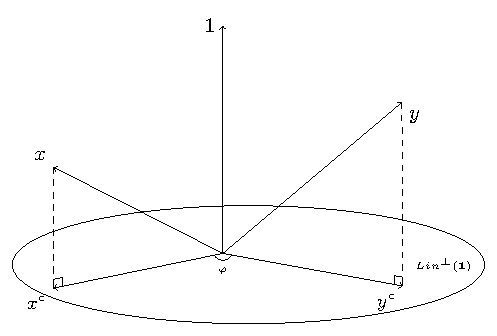
\includegraphics[scale=0.65]{figures/02_correlation_constant_centered_variables.pdf}
\caption{Centred vectors $x^c$ and $y^c$.}
\label{fig:corr_xyc}
\end{marginfigure}

Also note that the~angle $\varphi$ between the~original and centred vectors remains the~same.
The~result of this step is shown in Figure~\ref{fig:corr_xyc}.

Then we need to derive a new vector $\tilde x$ with constants added to each component.
Geometrically adding a vector of costants means adding a vector of all ones
scaled by $\alpha \in \mathbb{R}$, i.e., $\alpha \mathbf{1}$.
Then the new vector $\tilde x$ can be broken up into a sum of $\alpha \mathbf{1}$ and
$\beta x$, $\alpha, \beta \in \mathbb{R}$, which can be seen in Figure~\ref{fig:corr_final}.
After that we will project this new vector $\tilde x$ onto $\Lin^{\perp}(\mathbf{1})$.
By the properties of projection it is of no difference whether to project
the whole vector $\tilde x$ or project its parts $\alpha \mathbf{1}$
and $\beta x$ — the result is the same.
So, while $\beta x$ is projected onto the span of $x^c$, the projection of $\alpha \mathbf{1}$
onto the orthohgonal space $\Lin^{\perp}(\mathbf{1})$ yields zero as demonstrated
in Figure~\ref{fig:corr_final}.
Moreover, it follows that the angle between $\tilde x$ and $y$ is still $\varphi$.

\begin{figure}
\begin{center}
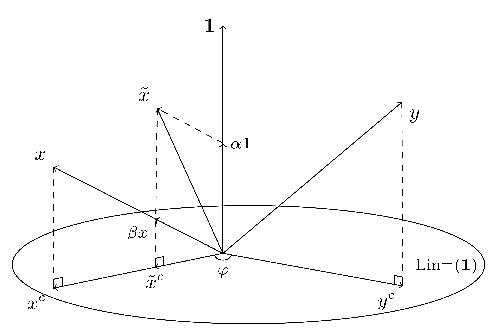
\includegraphics[width=0.6\linewidth]{figures/02_correlation_constant_proof.pdf}
\label{fig:corr_final}
\caption{$\sCorr(x + \alpha \mathbf{1}, y) = \sCorr(x,y)$ as the corresponding angles are equal.}
\end{center}
\end{figure}


Finally, putting everything together we finish the proof:
\[
\sCorr(x + \alpha \mathbf{1}, y) = \sCorr(x,y)
\]
\end{proof}


\subsection{Sample correlation coefficient in simple linear regression}

\begin{theorem}
A linear regression model with one explanatory variable and constant term
\[
y = \beta_1 \mathbf{1} + \beta_2 x + \varepsilon
\]
has the property
\[
\sCorr(y, \hat y) = \sign(\hat \beta_2) \sCorr(y, x)
\]
\end{theorem}

\marginnote{
Assuming the underlying relationship between $x$ and $y$ to be
\[
y_i = \beta_1 + \beta_2 x_i + \varepsilon_i \quad i=1,\ldots,n
\]
where $\varepsilon_i$ is an error term the following holds
\begin{align*}
\sCorr(y, \hat y) &= \frac{\sCov(y, \hat y)}{\sqrt{\sVar(y)\sVar(\hat y)}} \\
&= \frac{\sCov(y, \hat \beta_1 + \hat \beta_2 x)}{\sqrt{\sVar(y)\sVar(\hat \beta_1 + \hat \beta_2 x)}} \\
&= \frac{\sCov(y, \hat \beta_2 x)}{\sqrt{\sVar(y)\sVar(\hat \beta_2 x)}} \\
&= \frac{\hat \beta_2 \sCov(y, x)}{|\hat \beta_2| \sqrt{\sVar(y)\sVar(x)}} \\
&= \sign(\hat \beta_2) \frac{\sCov(y,x)}{\sqrt{\sVar(y)\sVar(x)}} \\
&= \sign(\hat \beta_2) \sCorr(y, x)
\end{align*}
}

\begin{proof}
Firstly, we consider the case when $\hat \beta_2 > 0$.
It has been shown earlier that the correlation coefficient represents the angle
between two random vectors.
So, in order to complete the proof we need to find the appropriate angles and compare them.

However, it seems to be difficult to compare the angles in the three dimensional space.
That is why we start with projecting both $x$ and $y$ onto the plane perpendicular to the vector of all ones (denoted as $\mathbf{1}$) as shown in Figure~\ref{fig:corr_pos_xyc}.
We denote this space as $\Lin^{\perp}(\mathbf{1})$. The resulting vectors are $x - \bar x \cdot \mathbf{1}$  and $y - \bar y \cdot \mathbf{1}$, respectively,
since projection of any vector $\vec{a}$ onto the span of a vector of all ones yields the vector of averages $\vec{\bar a}$.


In order to get the angle between $y$ and $\hat y$ we should start with regressing $y$ on $\Lin(x, \mathbf{1})$.
Then the only thing left is to project $\hat y$ onto $\Lin^{\perp}(\mathbf{1})$ since the $y$ vector has already been projected.
Note that the projected $\hat y$ falls onto tha span of vector $x - \bar x \cdot \mathbf{1}$ as it can be decomposed into a sum $a x + b \mathbf{1}$ where $a, b \in \mathbb{R}$.
The first component $a x$ is projected in the same way as $x$ and $b \mathbf{1}$ yields zero when projected onto the orthogonal space.
The result of this step is shown in Figure~\ref{fig:corr_pos_yhatc}.

\begin{figure*}[h!]
\begin{center}
\subfigure[]{
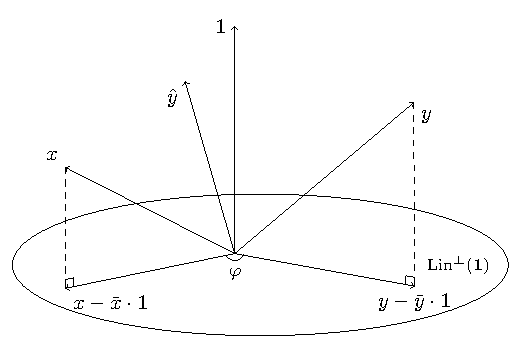
\includegraphics[width=0.45\linewidth]{figures/02_simple_regression_coefficient_centred_variables.pdf}
\label{fig:corr_pos_xyc}}
%\hspace{4ex}
\subfigure[]{
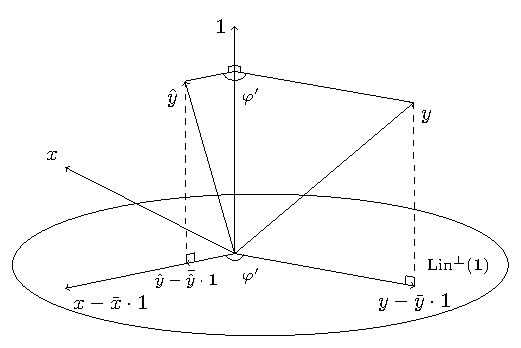
\includegraphics[width=0.45\linewidth]{figures/02_simple_regression_coefficient_yhat_projected.pdf}
\label{fig:corr_pos_yhatc}}
\caption{\subref{fig:corr_pos_xyc}: `Centred' $x$ and $y$, i.e., projected onto $\Lin^{\perp}(\mathbf{1})$;
\subref{fig:corr_pos_yhatc}: `Centred' $\hat y$, i.e., projected onto $\Lin^{\perp}(\mathbf{1})$.}
\end{center}
\end{figure*}

Since the projection of $\hat y$ lies exactly on the span of vector $x - \bar x \cdot \mathbf{1}$, we can conclude that $cos \varphi = \cos \varphi '$ and to put it another way $\sCorr(x,y) = \sCorr(y, \hat y)$.

Now consider the case when $\hat \beta_2 < 0$.
Note that the sign of $\beta_1$ does not influence the correlation coefficient sign.
The only difference is that now $\hat y$ is projected onto the span of  $x - \bar x \cdot \mathbf{1}$ and not on this vector itself while the projections of $x$ and $y$ remain the same.
Looking at Figure~\ref{fig:corr_negative} we deduce
that the~angle between $y$ and $\hat y$ is compelement to the angle between $x$ and $y$.
Using trigonometric properties, we simplify $\cos(180^{\circ} - \varphi) = -\cos\varphi$
which in turn implies $\sCorr(x,y) = -\sCorr(y,\hat y)$.

\begin{figure}[h!]
\begin{center}
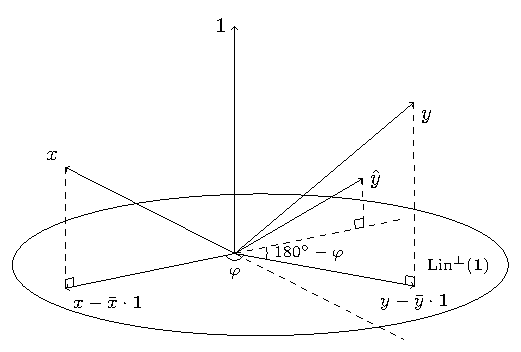
\includegraphics{figures/02_simple_regression_coefficient_negative.pdf}
\label{fig:corr_negative}
\caption{Case of $\beta_2 < 0$.}
\setfloatalignment{b}
\end{center}
\end{figure}
\end{proof}


\subsection{RSS + ESS = TSS}

\marginnote{
Consider a regression model with $n$ observations and $k$ explanatory variables
including a constant unit vector % unit?
\[
y = X \beta + \varepsilon
\]
The OLS estimator for the vector of coefficients $\beta$ is
\[
\hat \beta = (X^T X)^{-1} X^T y
\]
and the residual vector is
\begin{align*}
\hat e &= y - \hat y \\
&= y - X \hat \beta \\
&= y - X (X^T X)^{-1} X^T y
\end{align*}
Then we define residual sum of squares (RSS), explained sum of squares (ESS) and total sum of squares (TSS) as follows:
\begin{align*}
RSS &= \lVert y - \hat y \rVert^2_2 \\
ESS &= \lVert \hat y - \bar y \rVert^2_2 \\
TSS &= \lVert y - \bar y \rVert^2_2 \\
\end{align*}
}

\begin{theorem}
A linear regression model with $n$ observations and $k$ explanatory variables including a constant unit vector
\[
y = X \beta + \varepsilon
\]
has the following property
\[
RSS + ESS = TSS
\]
where $RSS = \lVert y - \hat y \rVert^2_2$, $ESS = \lVert \hat y - \bar y \rVert^2_2$, $TSS = \lVert y - \bar y \rVert^2_2$.
\end{theorem}

\begin{proof}
The proof will be presented for the case of two regressor $x$ and $\mathbf{1}$ in order for the picture to be clear.
However, the same logic applies for the case of $k$ regressors.

We start with depicting the vectors $y \in \mathbb{R}^{n-2}$ and $x, \mathbf{1} \in \mathbb{R}^2$.
Then we project $y$ onto $\Lin(x, \mathbf{1})$ and obtain $\hat y$ which is shown in Figure~\ref{fig:rss}.

From this picture we can immediately derive $\sqrt{RSS}$ as by definition this is the squared difference between $y$ and $\hat y$.

\begin{figure*}[h!]
\begin{center}
\subfigure[]{
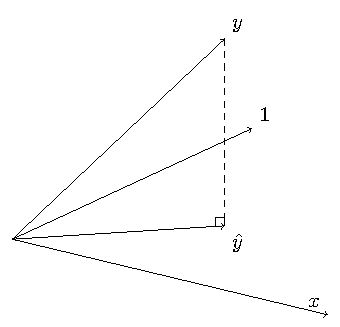
\includegraphics[width=0.3\linewidth]{figures/02_rss_ess_tss_yhat.pdf}
\label{fig:rss}}
\hspace{4ex}
\subfigure[]{
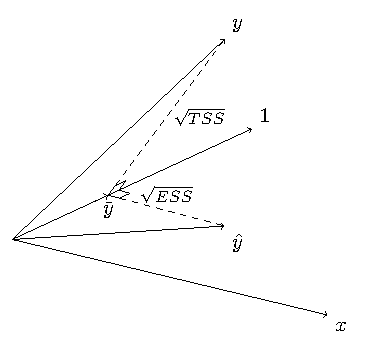
\includegraphics[width=0.3\linewidth]{figures/02_rss_ess_tss_sqr_tss_ess.pdf}
\label{fig:tss_ess}}
\subfigure[]{
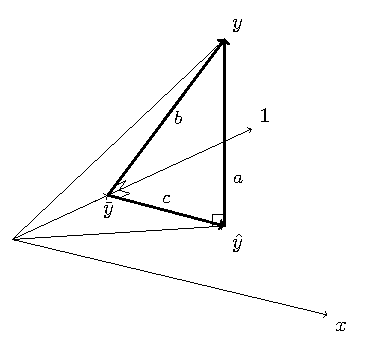
\includegraphics[width=0.3\linewidth]{figures/02_rss_ess_tss_final.pdf}
\label{fig:final}
}
\caption{\subref{fig:rss}: Residual sum of squares;
\subref{fig:tss_ess}: Total sum of squares and residual sum of squares;
\subref{fig:final}: Illustration of the equality $(\sqrt{RSS})^2 + (\sqrt{ESS})^2 = (\sqrt{TSS})^2$
where $a$ stands for $\sqrt{RSS}$, $b$ — $\sqrt{TSS}$, $c$ — $\sqrt{ESS}$.}
\end{center}
\end{figure*}

So as to visualize $ESS$ and $TSS$ we first need to visualize vector of averages $\bar y$.
Geometrically this means projecting a vector onto a line spanned by vector $\mathbf{1}$.

Now we both project $y$ and $\hat y$ onto $\mathbf{1}$ and following the definition obtain $\sqrt{TSS}$ as the difference vector $y - \bar y$ and $\sqrt{ESS}$ as the vector $\hat y - \bar y$.

The final step is to put everything together.
Note that since $y - \hat y$ is perpendicular to $\Lin(x, \mathbf{1})$ it is also perpendicular to $\hat y - \bar y$ and $\mathbf{1}$ as these vectoros are in $\Lin(x, \mathbf{1})$.
Then, applying the theorem of three perpendiculars we conclude that the foot of vector $y - \bar y$ is the same point as the foot of the vector $\hat y - \bar y$.
Thus, we obtain a right angle triangle and can apply the Pythagorean theorem for the catheti $\sqrt{RSS}$ and $\sqrt{ESS}$ and the
hypotenuse $\sqrt{TSS}$:
\[
\left(\sqrt{RSS}\right)^2 + \left(\sqrt{ESS}\right)^2 = \left(\sqrt{TSS}\right)^2
\]

\marginnote[-5\baselineskip]{
Disclosing parentheses and using the fact that $\hat{y}^T y = \hat{y}^T \hat{y}$
\begin{align*}
\hat{y}^T y &= \beta^T X^T y \\
&=  y^T X (X^T X)^{-1} X^T y \\
\hat{y}^T \hat{y} &= \beta^T X^T X \beta \\
&= y^T X (X^T X)^{-1} X^T X (X^T X)^{-1} X^T y \\
&= y^T X (X^T X)^{-1} X^T y
\end{align*}
we obtain
\begin{align*}
RSS &= y^T y -\hat{y}^T \hat{y} \\
ESS &= \hat{y}^T \hat{y} - \hat{y}^T \bar{y} + \bar{y}^T \bar{y} \\
TSS &= y^T y - 2 y^T \bar y +  \bar{y}^T \bar{y}
\end{align*}
When putting everything together all the terms cancel out which proves
\[
ESS + RSS = TSS
\]
}
\end{proof}

\vspace{3.5cm}
\subsection{Determination coefficient}

\marginnote[-2\baselineskip]{
\begin{align*}
\sCorr^2(y,\hat y) &= \left(\frac{\sCov(y, \hat y)}{\sqrt{\sVar(y)\sVar(\hat y)}}\right)^2 \\
&= \frac{\sCov(y, \hat y) \sCov(y, \hat y)}{\sVar(y)\sVar(\hat y)} \\
&= \frac{\sCov(\hat y + e, \hat y) \sCov(\hat y + e, \hat y)}{\sVar(y)\sVar(\hat y)} \\
&= \frac{\sCov(\hat y, \hat y) + \sCov(e, \hat y)}{\sVar(y)} \\
&\cdot \frac{\sCov(\hat y, \hat y) + \sCov(e, \hat y)}{\sVar(\hat y)} \\
&= \frac{\sVar(\hat y) \sVar(\hat y)}{\sVar(y)\sVar(\hat y)} \\
&= \frac{\sVar(\hat y)}{\sVar(y)} = \frac{ESS}{TSS} = R^2
\end{align*}
}

\begin{theorem}
A linear regression model with $n$ observations and $k$ explanatory variables including a constant unit vector
\[
y = X \beta + \varepsilon
\]
has the following property
\[
R^2 = \sCorr^2(y, \hat y)
\]
\end{theorem}

\begin{proof}
Proving this theorem geometrically means showing that the determination coefficient can be interpreted as some squared angle
which happens to be eqaul to the squared angle betwen $y$ and $\hat y$.

Consider Figure~\ref{fig:final} from the previous proof.
It was shown there that the vectors $y - \bar y$, $y - \hat y$ and $\hat y - \bar y$ form a right triangle.
Having defined the determination coefficient as
\[
R^2 = \frac{ESS}{TSS}
\]
we conclude that its geometric interpretaion is
\[
R^2 = \frac{ESS}{TSS} = \cos^2 \varphi
\]
as shown in Figure~\ref{fig:r_sq_angle}.

\begin{marginfigure}
  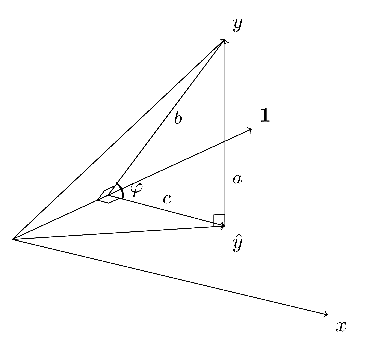
\includegraphics{figures/02_determination_coefficient.pdf}
  \caption{Determination coefficient as squared $\cos \varphi$
  where $a$ stands for $\sqrt{RSS}$, $b$ — $\sqrt{TSS}$, $c$ — $\sqrt{ESS}$.}
  \label{fig:r_sq_angle}
\end{marginfigure}

Recall that the sample correlation coefficient two vectors was defined earlier as the angle between these two vectors.
Thus, we conclude that $\sCorr(y, \hat y)$ is the angle between $y$ and $\hat y$ which is also eqaul to $\cos \varphi$.
Finally, squaring both sides, we obtain
\[
R^2 = \sCorr^2(y, \hat y)
\]
\end{proof}


\subsection{Regression line and point of averages}

\marginnote[-1\baselineskip]{
If the regression contains the intercept, the following equation holds:
\begin{align*}
\hat y  &= X \hat \beta = X (X^T X)^{-1} X^T y \\
&= X (X^T X)^{-1} X^T X \beta + X (X^T X)^{-1} X^T \varepsilon
\end{align*}
Premultiplying both sides by $X^T$, we obtain:
\begin{align*}
X^T \hat y &=  X^T X (X^T X)^{-1} X^T X \beta \\
&+ X^T X (X^T X)^{-1} X^T \varepsilon \\
&= X^T X \beta + X^T \varepsilon
\end{align*}
This is a system of equations. The first row of $X^T$ is $\mathbf{1}$ vector, so we can write out the first equation:
\[
\sum_{i=1}^n \hat y_i = \sum_{i=1}^{n} \sum_{j=1}^{k} x_{ij} \beta_{j}
\]
From the first equation in the system
\[
X^T \hat y = X^T y
\]
we obtain
\[
\sum_{i=1}^{n} \hat y_i = \sum_{i=1}^{n} y
\]
And this finishes the proof:
\[
\frac{1}{n} \sum_{i=1}^{n} y = \frac{1}{n} \sum_{i=1}^{n} \sum_{j=1}^{k} x_{ij} \beta_{j}
\]
}

\begin{theorem}
In a linear regression model with one explanatory variable and constant term
\[
y = \beta_1 + \beta_2 x + \varepsilon
\]
the point of averages lies on the estimated regression line.
\end{theorem}

\begin{proof}
For the geometrical proof it suffices to show that $\hat y$ is a linear combination of the regressors, which is true by construction,
and that $\frac{1}{n} \sum_{i=1}^{n} \hat y_i = \frac{1}{n} \sum_{i=1}^{n} y$. In order for the pictures to be more clear the proof will be presented for the case of two regressors.

The first step is regressing $y$ on $\Lin(\mathbf{1}, x)$. As shown in Figure~\ref{fig:averages_lin}, we obtain $\hat y$ as a linear combination of $\mathbf{1}$ and $x$.
The next step is to regress both $y$ and $\hat y$ on $\mathbf{1}$ which results in $\bar y$ and $\bar{\hat y}$ correspondingly.
By the theorem of three perpendiculars, $\bar y = \bar{\hat y}$ which is shown in Figure~\ref{fig:averages_bars}.

\begin{figure}[ht!]
\begin{center}
\subfigure[]{
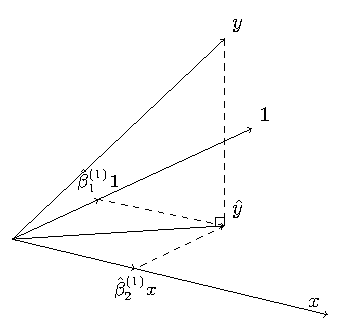
\includegraphics[width=0.35\linewidth]{figures/02_averages_yhat_decomposed.pdf}
\label{fig:averages_lin} }
\hspace{4ex}
\subfigure[]{
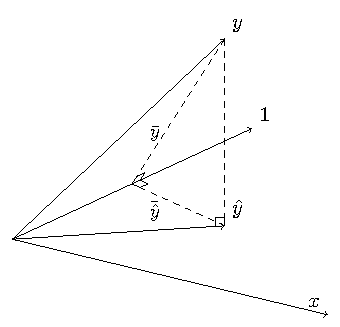
\includegraphics[width=0.35\linewidth]{figures/02_averages_final.pdf}
\label{fig:averages_bars}}
\caption{\subref{fig:averages_lin}: Regression of $y$ on $\Lin(\mathbf{1},x)$;
\subref{fig:averages_bars}: Regression of $y$ and $\hat y$ on $\mathbf{1}$.}
\setfloatalignment{b}
\end{center}
\end{figure}
\end{proof}


\subsection{Orthogonality of regressors}

\marginnote{
Consider a model
\[
y = \beta_1 x_1 + \beta_2 x_2 + \varepsilon
\]
with centred regressors $x_1$, $x_2$ such that $\bar x_1 = \bar x_2 = 0$.
Suppose we mistakenly believe in a model
\[
y = \beta_1^* x_1 + \varepsilon^*
\]
where $x_2$ is omitted. Then the new estimator
\begin{align*}
\E\left(\hat \beta_1^*\right) &= \E\left(\frac{\sCov(x_1, y)}{\sVar(x_1)}\right) \\
&= \E\left(\frac{\sCov(x_1, \beta_1 x_1 + \beta_2 x_2 + \varepsilon)}{\sVar(x_1)}\right) \\
&= \beta_1 + \beta_2 \frac{\sCov(x_1,x_2)}{\sVar(x_1)} + \E\left(\frac{\sCov(x_1, \varepsilon)}{\sVar(x_1)}\right) \\
&= \beta_1 + \beta_2 \frac{\sCov(x_1,x_2)}{\sVar(x_1)}
\end{align*}
will be unbiased if either $\beta_2 = 0$ or $\sCov(x1,x2) = 0$.
}

\begin{theorem}
Omitting a variable in a regression model does not lead to a bias in coefficient
estimators if either the coefficient of the omitted regressor equals zero
or the regressors are uncorrelated.
\end{theorem}

\begin{proof}
We will not consider the case when the coefficient of the omitted regressor
equals zero because this means that the model is not mis-specified.
The case of orthogonal regressors is less trivial.
However, it can be easily proved once the geometric approach is implemented.

\begin{marginfigure}
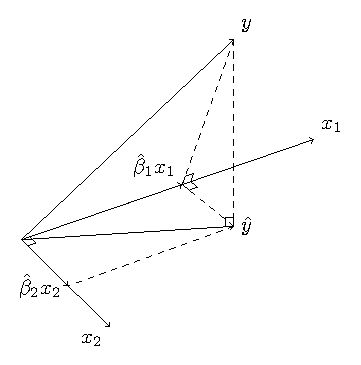
\includegraphics[scale=0.7]{figures/02_uncorrelated_regressors.pdf}
\label{fig:uncorrelated_regressors}
\caption{In case of uncorrelated regressors omitting one of them
does not result in bias of the estimator.}
\end{marginfigure}

Condider the following regression model
\[
y = \beta_1 x_1 + \beta_2 x_2 + \varepsilon
\]
where regressors $x_1$ and $x_2$ are uncorrelated, $x_1 \perp x_2$.
When we perform a regression of $y$ onto both $x_1$, $x_2$
we obtain predicted values $\hat y$ which can be broken up into a sum:
\[
\hat y = \hat \beta_1 x_1 + \hat \beta_2 x_2.
\]
Since $x_1$ and $x_2$ are orthogonal it folows that
the difference $\hat y - \hat \beta_1 x_1$ must be orthogonal to $x_1$.
Thus, by the theorem of three perpendiculars the projection of $y$ onto
$x_1$ also results in $\hat \beta_1 x_1$.
\end{proof}

\vspace{4cm}
\subsection{Geometry of formula for OLS estimators}

The following interpretation gives another view on the estimators obtained
by the ordianry least squares method.
Previously, we illustrated the ideas in the observations space, $\mathbb{R}^n$.
Apparantely, the OLS estimators can be depicted in the regressors space, $\mathbb{R}^k$.
This result follows from the Cramer's rule.

Consider a linear model with two regressors:
\[
\hat y = \hat \beta_1 x_1 + \hat \beta_2 x_2.
\]
Let us denote $X = \begin{pmatrix} x_1 \\ x_2 \end{pmatrix}$ and
$\langle X, y \rangle = \begin{pmatrix} \langle x_1,  y \rangle \\
\langle x_2,  y \rangle \end{pmatrix}$.
Then, taking scalar product, we obtain:
\[
\langle X, y \rangle = \hat \beta_1 \langle X, x_1 \rangle + \hat \beta_2 \langle X, x_2 \rangle
\]
All the elements of this equation are illustrated in Figure~\ref{fig:cramers}.

The area of each parallelogram is the determinant of the matrix with columns
which form the corresponding parallelogram.
For instance, the area of parallelogram formed by vectors $\langle X, y \rangle$, $\langle X, x_2 \rangle$
is equal to $\det([\langle X, y \rangle  \langle X,  x_2 \rangle])$.
The parallelogram formed by vectors $\langle X, \hat \beta_1 x_1 \rangle$,
$\langle X, x_2 \rangle$ has the area of $\hat \beta_1 \det([\langle X, x_1 \rangle  \langle X, x_2 \rangle])$.
Since both parallelograms must be of the same are we obtsin a formula for $\hat \beta_1$:
\[
\hat \beta_1 = \frac{\det([\langle X, y \rangle  \langle X,  x_2 \rangle])}{ \det([\langle X, x_1 \rangle  \langle X, x_2 \rangle])}.
\]

\begin{marginfigure}
  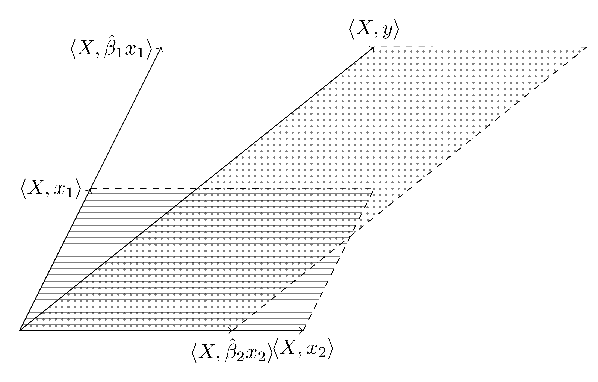
\includegraphics[scale=0.5]{figures/02_cramers_rule.pdf}
  \label{fig:cramers}
  \caption{Illustration of estimators in $\mathbb{R}^k$ as the ratio of parallelogram areas.}
\end{marginfigure}

So as to generalize this result we introduce a matrix $A = (y | X)$
that has $y$ as its first column and all the regressors as the rest ones.
We will denote this matrix without column $y$ or $x$ as $A_{-y}$, $A_{-x}$, respectively.
Then, we can write out the formula for $\beta_x$:
\[
\hat \beta_x = \frac{\det(\langle A_{-y}, A_{-x} \rangle)}{\det(\langle A_{-y}, A_{-y} \rangle)}.
\]

If there is a regression with unit vector among the regressors and
the Frisch-Waugh-Lovell theorem is applied, the formula above takes the followin form:
\[
\hat \beta_x = \frac{\det(\sCov(A_{-y}, A_{-x}))}{\det(\sVar(A_{-y}))}.
\]


\subsection{Frisch–Waugh–Lovell theorem}

\marginnote{From regression~(\ref{eq:fwl_2}) we get the following estimator:
\begin{align*}
\hat\beta_2 &= ((M_1 X_2)^T M_1 X_2)^{-1}(M_1 X_2)^T M_1 y \\
&= (X_2^T M_1^T M_1 X_2)^{-1}  X_2^T M_1^T M_1 y \\
&= (X_2^T M_1 X_2)^{-1}  X_2^T M_1 y
\end{align*}
As for regression~(\ref{eq:fwl_1}), let us note that due to $y = \hat y + \hat u$ $y$ can be decomposed as follows:
\[
y = Py + My = X_1 \hat \beta_1 + X_2 \hat \beta_2 + My
\]
Premultiplying both sides by $X_2^T M_1$, we obtain:
\begin{align*}
X_2^T M_1 y &= X_2^T M_1 X_1 \hat\beta_1 + X_2^T M_1 X_2 \hat\beta_2 + X_2^T M_1 M y \\
&=  X_2^T M_1 X_2 \hat\beta_2 + X_2^T M_1 M y \\
&= X_2^T M_1 X_2 \hat\beta_2
\end{align*}
On the last step we used the fact that
\begin{align*}
(X_2^T M_1 M y)^T = y^T M^T M_1^T X_2 \\
= y^T M M_1 X_2 = y^T M X_2 = 0^T
\end{align*}
Assuming $X_2^T M_1 X_2$ is invertible, we get the same estimator
\[
\hat\beta_2 = (X_2^T M_1 X_2)^{-1}  X_2^T M_1 y
\]
}

\begin{theorem}
Consider regression
\begin{equation} \label{eq:fwl_1}
y = X_1 \beta_1 + X_2 \beta_2 + u
\end{equation}
where $X_{n \times k} = [X_1 X_2]$, i.e. $X_1$ consists of first $k_1$ columns of $X$ and $X_2$ consists of remaining $k_2$ columns of $X$,
$\beta_1$ and $\beta_2$ are comformable, $k_1 \times 1$ and $k_2 \times 1$ vectors.
Consider another regression
\begin{equation}  \label{eq:fwl_2}
M_1 y = M_1 X_2 \beta_2 + M_1 u
\end{equation}
where $M_1 = I - P_1$ projects onto the~orthogonal complement of the~column space~of
$X_1$ and $P_1 = X_1(X_1^TX_1)^{-1}X_1^T$ is the~projection onto the~column space of~$X_1$.
Then the~estimate of $\beta_2$ from regression~(\ref{eq:fwl_1}) will be the~same
as the~estimate from regression~(\ref{eq:fwl_2}).
\end{theorem}

There are two ways to~visualize the~proof of~the~Frisch-Waugh-Lovell theorem
using geometric concepts. Both are presented below.

\begin{proof}
1.~Consider the following model:
\begin{equation} \label{eq:fwl_proof}
y_i = \beta_1 x_i + \beta_2 z_i + u_i
\end{equation}

We start with a `one-step' regression  and will distinct its coefficients with
an upper index $A$.
The~only step in~obtaining $\beta_1^{A}$ is regressing $y$ on~$\Lin(x,z)$ and
then expanding $\hat y$ as a~linear combination of~basis vectors $x$ and $z$,
which is shown in~Figure~\ref{fig:fwl_1_regression_3d}. Figure~\ref{fig:fwl_1_regression_lin}
depicts $\Lin(x, z)$.

\begin{figure}[ht!]
\begin{center}
\subfigure[]{
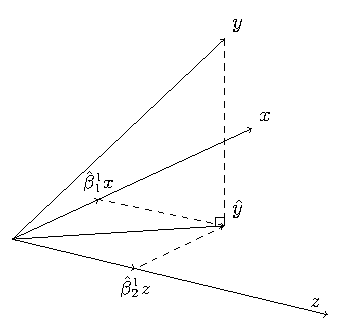
\includegraphics[width=0.4\linewidth]{figures/02_fwl_v1_yhat_decomposed.pdf}
\label{fig:fwl_1_regression_3d}}
\hspace{4ex}
\subfigure[]{
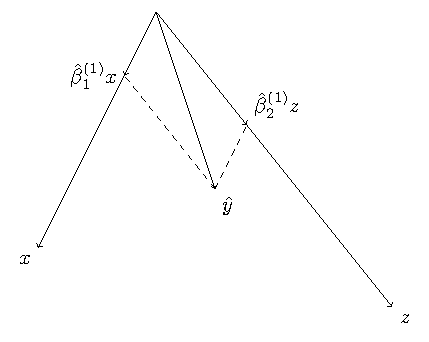
\includegraphics[width=0.4\linewidth]{figures/02_fwl_v1_yhat_decomposed_lin.pdf}
\label{fig:fwl_1_regression_lin}}
\caption{\subref{fig:fwl_1_regression_3d}: Regression of $y$ on $\Lin(x,z)$;
\subref{fig:fwl_1_regression_lin}: $\Lin(x, z)$.}
\end{center}
\end{figure}

As for the~model~(\ref{eq:fwl_2}) where several regressions are performed consecutively
we start with regressing $y$~on~$z$, resulting in $\tilde{y}$,
which we will refer~to as~`cleansed' $y$.
We will denote its coefficients with an upper index $B$.

\begin{equation}\label{eq:fwl_2_y_clean}
\begin{aligned}
y &= \alpha z + \varepsilon \\
\hat\alpha &= \frac{y^T z}{z^T z} \\
\tilde{y} &= \hat\varepsilon = y - \frac{y^T z}{z^T z}z
\end{aligned}
\end{equation}

Following that, $x$ is regressed on $z$, resulting in $\tilde{x}$ — `cleansed' $x$.

\begin{equation}\label{eq:fwl_2_x_clean}
\begin{aligned}
x &= \gamma z + \nu \\
\hat\gamma &= \frac{x^T z}{z^T z} \\
\tilde{x} &= \hat\nu = x - \frac{x^T z}{z^T z}z
\end{aligned}
\end{equation}

Geometric results of these two steps are presented in~\ref{fig:fwl_2_regression_first}.

Finally, `cleansed' $y$ must be regressed on `cleansed' $x$.
However, it cannot be performed immediately as $\tilde{y}$ and $\tilde{x}$ are skew lines.
So at first, we fix this problem by translation and after that obtain
$\hat\beta_1^{B}\tilde x$ (see Figure~\ref{fig:fwl_2_regression_trans}).

\begin{figure}[ht!]
\begin{center}
\subfigure[]{
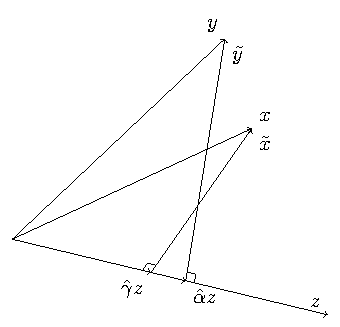
\includegraphics[width=0.4\linewidth]{figures/02_fwl_v1_cleansed_variables.pdf}
\label{fig:fwl_2_regression_first} }
\hspace{4ex}
\subfigure[]{
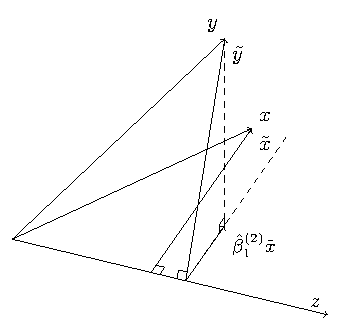
\includegraphics[width=0.4\linewidth]{figures/02_fwl_v1_translation.pdf}
\label{fig:fwl_2_regression_trans}}
\caption{\subref{fig:fwl_2_regression_first}: Regression of $y$ on $z$ and of $x$ on $z$;
\subref{fig:fwl_2_regression_trans}: Translation of $\tilde{x}$.}
\end{center}
\end{figure}

Now let us picture all the results in one figure and mark some main points.

\begin{figure}[ht!]
\begin{center}
\subfigure[]{
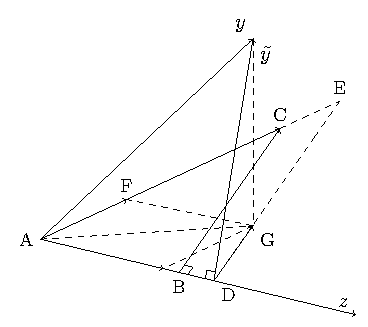
\includegraphics[width=0.4\linewidth]{figures/02_fwl_v1_final.pdf}
\label{fig:fwl_3_3d} }
\hspace{4ex}
\subfigure[]{
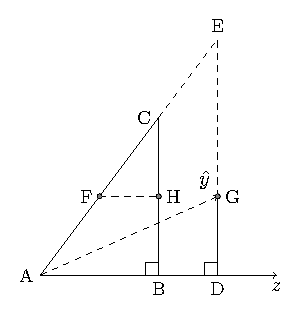
\includegraphics[width=0.4\linewidth]{figures/02_fwl_v1_final_lin.pdf}
\label{fig:fwl_3_lin}}
\caption{\subref{fig:fwl_3_3d}: Point A stands for the origin, B — $\hat\gamma z$,
C — $x$, D — $\hat\alpha z$, E — intersection of vector $x$ and line parallel to $\tilde x$,
F — $\hat\beta_1^{A} x$, G — $\hat\beta_1^{B} \tilde{x}$; \subref{fig:fwl_3_lin}: $\Lin(x,z)$.}
\end{center}
\end{figure}

In Figure~\ref{fig:fwl_3_lin} segments $AF$ and $BH = DG$ stand for $\hat\beta_1^{A}x$
and $\hat\beta_1^{B}\tilde x$ respectively, while segments AC and BC represent $x$ and $\tilde{x}$.
Having two congruent angles, triangles ABC and FHC are simillar.
Then, it follows:
\[
\frac{AF}{AC} = \frac{BH}{BC} \Leftrightarrow \frac{\hat\beta_1^{A}x}{x} = \frac{\hat\beta_1^{B}\tilde x}{\tilde x} \Leftrightarrow \hat\beta_1^{A} = \hat\beta_1^{B}
\]

2. Alternatively, we could implement a~concept close to the~partial correlation.
In the~same model~(\ref{eq:fwl_proof}) we wiil treat $z$ vector fixed and again
consecutively cleanse the $x$ and $y$ variables by projecting them onto
the~space orthogonal to $z$, i.e., $\Lin^\perp(z)$ as demonstrated in Figure~\ref{fig:fwl_v2_rcleansed}.
Then we perform a~regression of the~`cleansed' $\tilde y$ on the~`cleansed' $\tilde x$
(see Figure\ref{fig:fwl_v2_regression_cleansed}).

\begin{figure}[ht!]
\begin{center}
\subfigure[]{
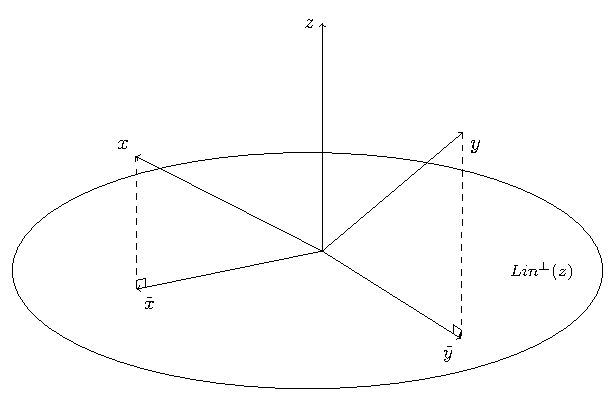
\includegraphics[width=0.45\linewidth]{figures/02_fwl_v2_cleansed_variables.pdf}
\label{fig:fwl_v2_rcleansed}}
\subfigure[]{
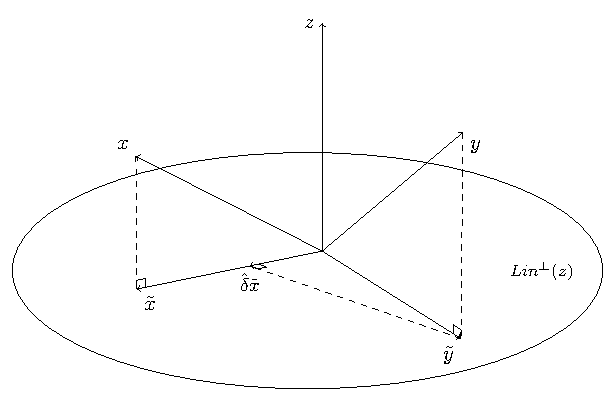
\includegraphics[width=0.45\linewidth]{figures/02_fwl_v2_cleansed_regression.pdf}
\label{fig:fwl_v2_regression_cleansed}}
\caption{\subref{fig:fwl_2_regression_first}: `Cleansed' variables $\tilde x$ and $\tilde y$;
\subref{fig:fwl_2_regression_trans}: `Cleansed' $\tilde y$ regressed on `cleansed' $\tilde{x}$.}
\end{center}
\end{figure}

Now we show that the~latter regression produces $\hat \beta_1$ coefficient which
is exactly the~coefficient from the~`one-step' regression of~original $y$ onto
original $x$ and $z$. Recall that the~vector $y$ can be split~up into a~sum of
some multiple of $x$ and some multiple of $z$. Since the second term is
the~orthogonal component its projection yields zero. The~multiple of $x$
is equal to $\hat \beta_1$ by construction.

Assume that the~coefficient at~$\tilde x$ is some unknown variable $\hat \delta$.
Then consider the~similar triangles in the $\Lin(x,z)$. From the~proportions
we obtain:
\[
\frac{CE}{CA} = \frac{CD}{CB} \Leftrightarrow \frac{\hat \beta_1 x}{x} = \frac{\hat \delta \tilde x}{\tilde x} \Rightarrow \hat \beta_1 = \hat \delta
\]

\begin{figure}[ht!]
\begin{center}
\subfigure[]{
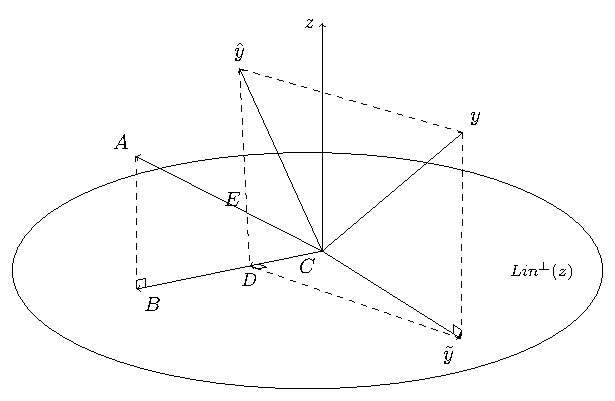
\includegraphics[width=0.45\linewidth]{figures/02_fwl_v2_similar_triangles.pdf}
\label{fig:fwl_v2_triangles}}
\subfigure[]{
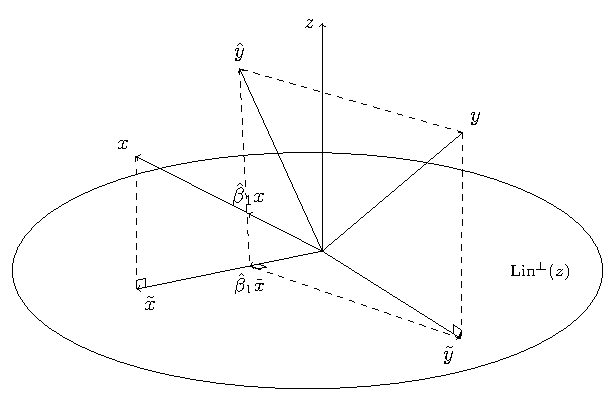
\includegraphics[width=0.45\linewidth]{figures/02_fwl_v2_final.pdf}
\label{fig:fwl_v2_final}}
\caption{\subref{fig:fwl_2_regression_first}: Similar triangles: $\bigtriangleup ABC \sim \bigtriangleup EDC$;
\subref{fig:fwl_2_regression_trans}: Alternative proof for the Frisch-Waugh-Lovell theorem.}
\end{center}
\end{figure}
\end{proof}


\subsection{Duality of regressors and residuals}

The idea of duality is widely used in mathematics.
The concept is to apply some transformation twice and get the~original object.
For example, if $f(a) = 1/a$:
\[
x \stackrel{f}{\to} \frac{1}{x} \stackrel{f}{\to} \frac{1}{1/x} = x
\]
We show that there is duality between regressors and residuals.

\begin{theorem}
Let $x_i$ be a $n \times 1$ regressor,
$u_i$ — a residual in regression of $x_i$ on all the rest regressors,  $i = 1, \ldots, k$.
Consider a transformation of a vector $v$, $f(v) = v/\lVert v \rVert^2$.
Then applying this transformation on the residuals $u_1, \ldots, u_k$ yields
new regressors $v_1, \ldots, v_k$.
Performing $k$ regressions of each $v_i$ on all the rest regressors and
applying the same transformation to the new residuals results in
the original regressors $x_1, \ldots, x_k$.
\end{theorem}

\begin{proof}

\begin{marginfigure}[-2\baselineskip]
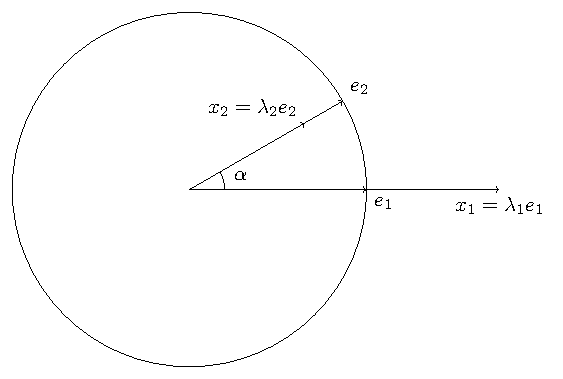
\includegraphics[scale=0.7]{figures/02_duality_original_regressors.pdf}
\caption{Two regressors in the unit circle.}
\end{marginfigure}

We start with $2$-dimensional case with two regressors,
and discuss the~case of spaces of higher dimensions later.

As stated in the~theorem we need to keep the~measure of the~lengths of the~regressors.
In order to do this we choose a~basis in $\mathbb{R}^2$ in such a~way that
\begin{align*}
&x_1 = \lambda_1 e_1, \quad \lVert e_1 \rVert = 1 \\
&x_2 = \lambda_2 e_2, \quad \lVert e_2 \rVert = 1
\end{align*}
where $\lambda_1, \lambda_2 \in \mathbb{R}$.

\begin{marginfigure}
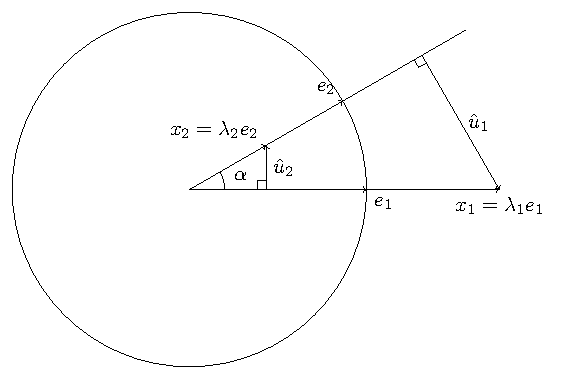
\includegraphics[scale=0.7]{figures/02_duality_first_residuals.pdf}
\label{fig:duality_fst_residuals}
\caption{Residuals $\hat{u}_1$ and $\hat{u}_2$.}
\end{marginfigure}

Then we perform two regressions
\begin{align*}
&x_1 = \beta_1 x_2 + u_1 \\
&x_2 = \beta_2 x_1 + u_2
\end{align*}
and get the residuals $\hat{u}_1$, $\hat{u}_2$.
Being orthogonal to $x_2$ and $x_1$, correspondingly, they can be written as follows
\begin{align*}
&\hat{u}_1 = \sin \alpha \cdot \lambda_1 \tilde{e}_1, \quad \lVert \tilde{e}_1 \rVert = 1 \\
&\hat{u}_2 = \sin \alpha \cdot \lambda_2 \tilde{e}_2, \quad \lVert \tilde{e}_2 \rVert = 1
\end{align*}
where $\tilde{e}_1 \perp e_2$ and $\tilde{e}_2 \perp e_1$.

For convenience we translate all the vectors $x_1$, $x_2$, $\hat{u}_1$, $\hat{u}_2$
to the origin of the unit circle as shown in Figure~\ref{fig:duality_fst_residuals_translated}
and after that we invert them.

\begin{marginfigure}
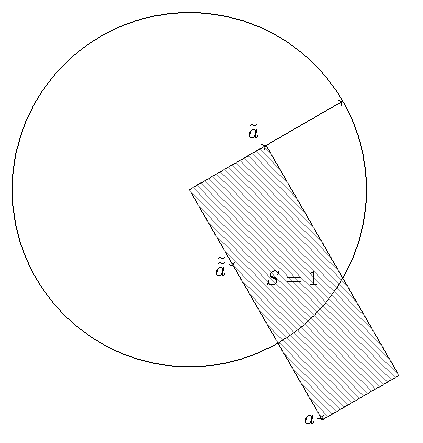
\includegraphics[scale=0.7]{figures/02_duality_inversion.pdf}
\label{fig:duality_inversion}
\caption{Example of inversion for vector $a$.}
\end{marginfigure}

In order to illustrate inversion consider an example with an arbitrary vector $a$.
Knowing its length, the aim is to find such an orthogonal vector $\tilde a$
that the product $\lVert a \rVert^2 \cdot \lVert \tilde a \rVert^2 = 1$.
In other words, we need to find an edge of rectangle with area equal to $1$.
Solving for $\tilde a$, we obtain the length of the inverted vector $a$.
The only thing left is to rotate this inverted vector back
to get a vector $\tilde{\tilde a}$ which satisfies both
\begin{align*}
& \lVert \tilde{\tilde a} \rVert^2 = \frac{1}{\lVert a \rVert^2} \\
& \cos(a, \tilde{\tilde a}) = 1
\end{align*}

\marginnote[-2\baselineskip]{
The transformation stated in the theorem is $f(v) = v / \lVert v \rVert^2$.
Generally speaking, $g(v) = v / (c \cdot \lVert v \rVert^2)$ where $c \in \mathbb{R}$
would also work.
\begin{multline*}
v \stackrel{g}{\to} \frac{v}{c \cdot \lVert v \rVert^2} = w \stackrel{g}{\to} \\
\frac{w}{c \cdot \lVert w \rVert^2} = \frac{\frac{v}{c \cdot \lVert v \rVert^2}}{c \frac{\lVert v \rVert^2}{c^2 \lVert v \rVert^4}} = v
\end{multline*}
}

Having applied the inversion to $\hat{u}_1$, $\hat{u}_2$, we obtained
new vectors $y_1$, $y_2$. Moreover, there is an algebraic expression for them
in terms of rotated basis $\tilde{e}_1$, $\tilde{e}_2$:
\begin{align*}
&\hat{u}_1 = \sin \alpha \cdot \lambda_1 \tilde{e}_1 \Rightarrow y_1 = \frac{1}{\sin \alpha \cdot \lambda_1} \tilde{e}_1 \\
&\hat{u}_2 = \sin \alpha \cdot \lambda_2 \tilde{e}_2 \Rightarrow y_2 = \frac{1}{\sin \alpha \cdot \lambda_2} \tilde{e}_2 \\
\end{align*}

Next, we perform another two regressions:
\begin{align*}
& y_1 = \gamma_1 y_2 + v_1 \\
& y_1 = \gamma_2 y_1 + v_2
\end{align*}

\begin{figure*}[ht!]
\begin{center}
\subfigure[]{
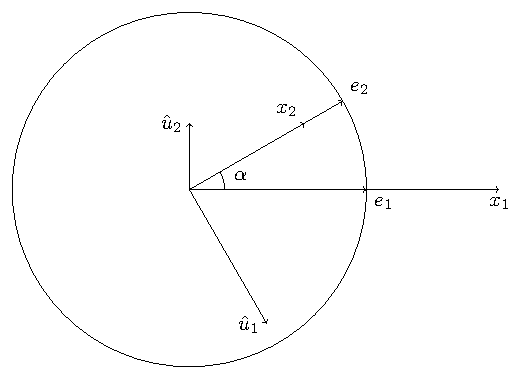
\includegraphics[width=0.3\linewidth]{figures/02_duality_first_residuals_translated.pdf}
\label{fig:duality_fst_residuals_translated}}
\subfigure[]{
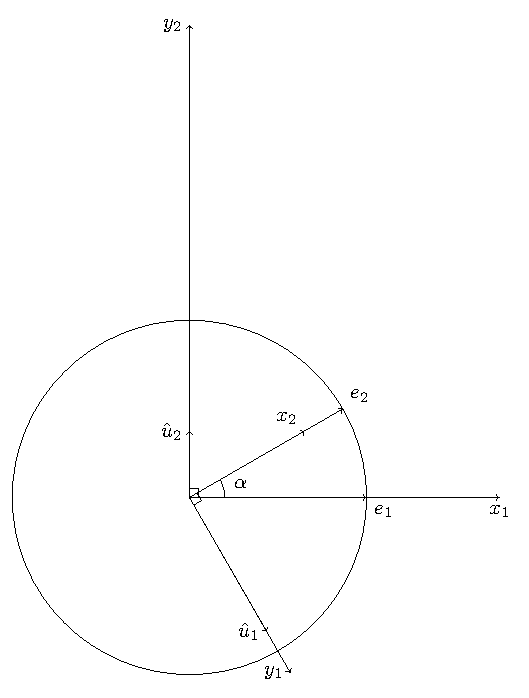
\includegraphics[width=0.3\linewidth]{figures/02_duality_new_regressors.pdf}
\label{fig:duality_new_regreesors}}
\subfigure[]{
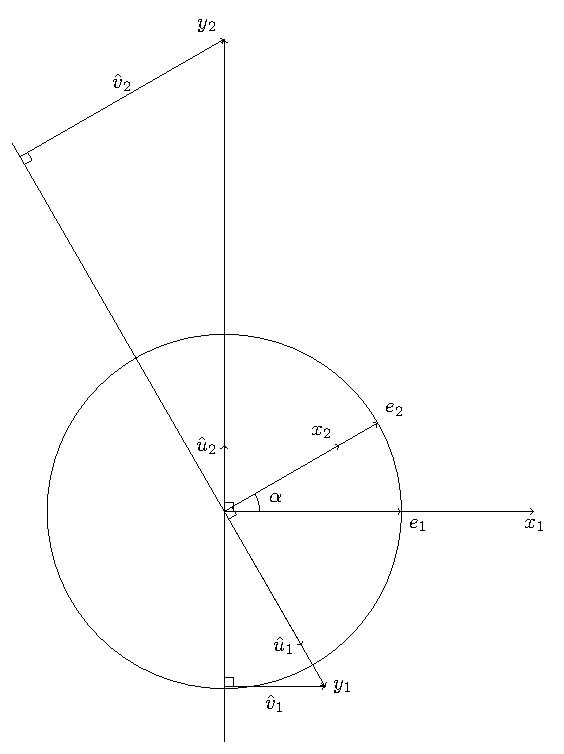
\includegraphics[width=0.3\linewidth]{figures/02_duality_new_residuals.pdf}
\label{fig:duality_new_residuals}}
\caption{\subref{fig:duality_fst_residuals_translated}: Residuals translated to the orgin of the unit circle;
\subref{fig:duality_new_regreesors}: Regressors $v_1$, $v_2$ obtained from inversion of the residuals $\hat{u}_1$, $\hat{u}_2$;
\subref{fig:duality_new_residuals}: Regressions of $v_1$ onto $v_2$ and of $v_2$ onto $v_1$.}
\end{center}
\end{figure*}

There are two things to notice about the new residuals $\hat{v}_1$, $\hat{v}_2$.
First, $\hat{v}_1$ is perpendicular to the line spanned by $\tilde{e}_2$.
Similarly, $\hat{v}_2$ is perpendicular to the line spanned by $\tilde{e}_1$.
This means, that they are parallel to $e_1$, $e_2$, correspondingly,
and once translated, they can be expressed as a multiple of $x_1$, $x_2$.

Second, we can find the lengths of these new residuals from the~right
triangles depicted in Figure~\ref{fig:duality_new_residuals}:
\begin{align*}
& \lVert \hat{v}_1 \rVert = \sin \alpha \cdot \lVert y_2 \rVert = \sin \alpha \cdot \left\lVert \frac{1}{\sin \alpha \cdot \lambda_1} \tilde{e}_1 \right\rVert = \frac{1}{\lambda_1} \\
& \lVert \hat{v}_2 \rVert = \sin \alpha \cdot \lVert y_1 \rVert = \sin \alpha \cdot \left\lVert \frac{1}{\sin \alpha \cdot \lambda_2} \tilde{e}_2 \right\rVert = \frac{1}{\lambda_2}
\end{align*}
Thus, when translated to the origin, the new resiuduals can be rewritten as
\begin{align*}
& \hat{v}_1 = \frac{1}{\lambda_1} e_1 \\
& \hat{v}_2 = \frac{1}{\lambda_2} e_2
\end{align*}

\begin{marginfigure}[4\baselineskip]
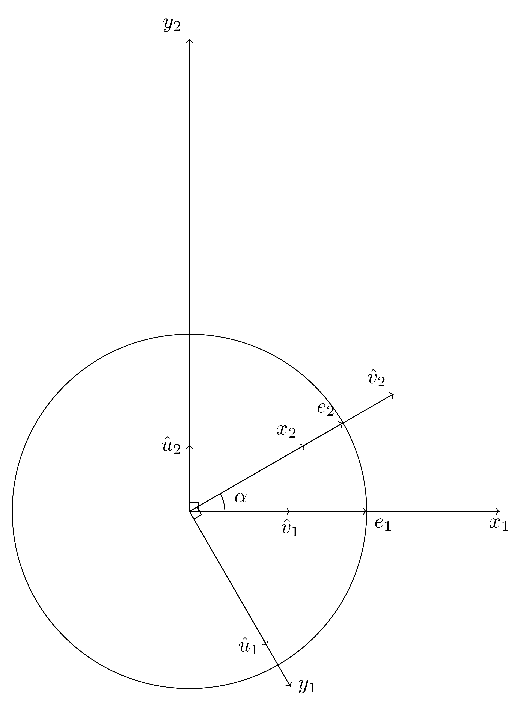
\includegraphics[scale=0.6]{figures/02_duality_final.pdf}
\label{fig:duality_final}
\caption{New residuals translated to the origin of the unit circle.}
\end{marginfigure}

The last step is to invert $\hat{v}_1$, $\hat{v}_2$.
Following the same procedure as described above, we finally get the desired result:
\begin{align*}
& \hat{v}_1 = \frac{1}{\lambda_1} e_1 \to \lambda_1 e_1 = x_1 \\
& \hat{v}_2 = \frac{1}{\lambda_2} e_2 \to \lambda_2 e_2 = x_2
\end{align*}
\end{proof}

\vspace{3.5cm}
\subsection{Gauss-Markov theorem}

\begin{theorem}
In the homoskedastic linear regression model the best (minimum-variance) linear
unbiased estimator is given by the ordinary least squares.
\end{theorem}


\begin{proof}

Consider an OLS estimator and an alternative one:
\begin{align*}
\hat{\beta}_{OLS} &= (X^T X)^{-1} X^T y = A^T y \\
\hat{\beta}_{alt} &= A^T_{alt} y
\end{align*}

% Hansen
\marginnote[-4\baselineskip]{
Consider an estimator $\beta$ which is a linear function of $Y$:
\[
\hat \beta = A^T Y
\]
where $A$ is an $n \times k$ function of $X$ such that $A^T X = I_k$.
From
\begin{align*}
\Var(\hat\beta_{OLS}) &= (X^T X)^{-1} \sigma^2 \\
\Var(A^T y) &= A^T A \sigma^2
\end{align*}
it follows that it is sufficient to prove that $A^T A - (X^T X)^{-1}$
is positive semi-definite. Set $C = A - X(X^T X)^{-1}$ and note that $X^T C = 0$, then
\begin{multline*}
A^T A - (X^T X)^{-1} \\
= (C + X(X^T X)^{-1})^T (C + X(X^T X)^{-1}) - (X^T X)^{-1} \\
= C^T C + C^T X(X^T X)^{-1} + (X^T X)^{-1} X^T C + \\
(X^T X)^{-1} X^T X(X^T X)^{-1} - (X^T X)^{-1} \\
= C^T C
\end{multline*}
Matrix $C^T C$ is positive semi-definite since
\[
\forall a \not= 0 \qquad a^T C^T C a = \lVert C a \rVert^2 \geq 0
\]
}

Note that $A^T X = I_{k}$, then the following holds for all $\beta$:
\begin{align*}
A^T X \beta &= \beta \\
A^T_{alt} X \beta &= \beta
\end{align*}
Taking the difference of these equations, we obtain:
\[
\left(A^T_{alt} - A^T\right) X \beta = 0 \Rightarrow \left(A^T_{alt} - A^T\right) \perp X
\]
If we treat the coefficients separately and consider, for instance, $\beta^{(2)}$,
we get the following result
\[
\left(a^T_{alt} - a^T\right) \perp X
\]
where $a_{alt}$ and $a$ are the second columns of matrices
$A_{alt}$ and $A$ correspondingly.
Since $a \in \Lin(\col X)$, it follows that $a_{alt} \not \in \Lin(\col X)$.

\begin{marginfigure}[1\baselineskip]
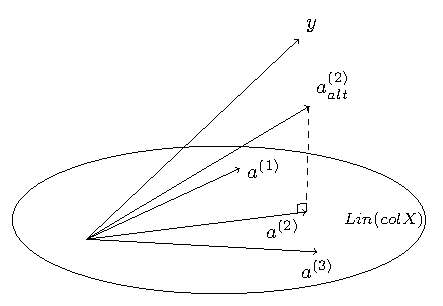
\includegraphics[scale=0.7]{figures/02_gmt.pdf}
\label{fig:gmt}
\caption{Gauss-Markov theorem for the case of three regressors
where $a^{(1)}$, $a^{(2)}$, $a^{(3)}$ are columns of matrix $A$.}
\end{marginfigure}

Now we can express the variances of both estimators in terms of $a_{alt}$ and $a$:
\begin{align*}
\Var\left(\hat{\beta}^{(2)}_{OLS}\right) &= \Var\left(a^T y\right) = a^T \sigma^2 I_{k} a = \sigma^2 \left\lVert a \right\rVert^2 \\
\Var\left(\hat{\beta}^{(2)}_{alt}\right) &= \Var\left(a^T_{alt} y\right) =  a^T_{alt} \sigma^2 I_{k} a_{alt} = \sigma^2 \left\lVert a_{alt} \right\rVert^2
\end{align*}
Since vectors $a$, $a_{alt}$ and $a - a_{alt}$
form a right triangle and $a_{alt} \not \in \Lin(\col X)$,
the vector $\left\lVert a_{alt} \right\rVert^2$ must be longer than $a$,
and the corresponding estimator must have higher variance.

\end{proof}

\vspace{1cm}

\subsection{Geometry of instrumental variables}

Consifder a model with an endogenity problem, i.e. explanotary variable $x$
is correlated with the error term $u$:
\[
y = \beta x + u
\]
Assume there is an instrument $z$ which is dependent with the problematic regressor $x$
but uncorrelated with the error term $u$.
The 2SLS procedure tells us to perform the following steps.
\begin{enumerate}
  \item Regress $x$ onto $z$ and get the vector of predicted values $\hat x$,
  \item Regress $y$ onto $\hat x$.
\end{enumerate}
These steps result in $\beta_{IV}$ estimator which is illustrated in Figure~\ref{fig:instrumental}.

The same result could be obtained with the oblique projection.
That is projecting $y$ onto $x$ along the vector perpendicular to the span of $z$.

\begin{marginfigure}[10\baselineskip]
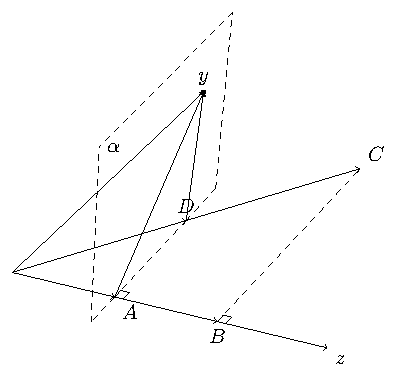
\includegraphics[scale=0.85]{figures/02_instr.pdf}
\caption{Geometry of instrumental variables. $A$ stands for $\hat \beta_{IV} \hat x$,
$B$ — $\hat x$, $C$ — $x$, $D$ — $\hat \beta_{IV} x$.}
\label{fig:instrumental}
\end{marginfigure}

The equivalence of these two methods holds due to the similarity of triangles.
Consider a plane $\alpha$ which satisfies the property of being perpendicular
to the span of $z$, $\alpha \perp z$.
Vectors $x$, $z$ and $\hat x$ form a triangle which is denoted as $\bigtriangleup OBC$
where $\overrightarrow{OB} = \hat{x}$, $\overrightarrow{OC} = x$.
In order to get an oblique projection of $y$ onto $x$ we could either
project $y$ directly onto $x$ staying in the plane $\alpha$
or get the same result in two steps. First, project $y$ onto $z$
and then project the result onto $x$ which gives the same outcome
by the theorem of three perpendiculars. Thus, we get another triangle $\bigtriangleup OAD$
where $\overrightarrow{OA} = \hat \beta_{IV} \hat x$, $\overrightarrow{OD} = \hat \gamma x$.
Since triangles $\bigtriangleup OBC$ and $\bigtriangleup OAD$ are similar
it follows that
\[
\frac{OD}{OC} = \frac{OA}{OB}
\]
which means that
\[
\hat \gamma = \hat \beta_{IV}.
\]


\subsection{Geometry of proxy variables}

Consider a model
\[
y = \beta_1 x + \beta_2 w + u
\]
where the error term $u$ is not correlated with the regressors.
Suppose that $w$ is an unobservable variable.
One way to deal with this problem and get a consistent estimator of $\beta_1$ is to use a proxy variable.
In order to clearly state its properties we decompose the unobservable variable
into a sum of a multiple of the proxy ($pr$) and a part that is uncorrelated
with the proxy ($\hat \nu$):
\[
\hat w = \gamma \cdot pr + \hat \nu
\]
Then the proxy variable must satisfy the following properties.
\begin{enumerate}
  \item It must be correlated with the unobservable variable $w$, $pr \not\perp w$.
  \item The error term $\hat u$ must be uncorrelated with the proxy variable, $pr \perp \hat u$.
  \item The error term $\hat \nu$ must be uncorrelated with the regressor $x$, $x \perp \hat \nu$.
\end{enumerate}

\begin{marginfigure}
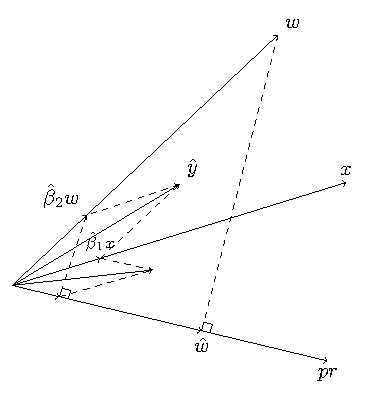
\includegraphics[scale=0.85]{figures/02_proxy.pdf}
\caption{Geometry of proxy variables.}
\label{fig:proxy}
\end{marginfigure}

To get a consistent estimator of $\beta_1$ we need to regress $y$ onto $x$ and $pr$.
Consistency is illustarted in Figure~\ref{fig:proxy}.
Suppose we could get the $\hat y$ by performing the original regression of
$y$ onto $x$ and $w$. Then, $\hat y$ could be decomposed in a sum of
$\hat \beta_1 x$ and $\hat \beta_2 w$.
Notice, that $\hat y$ is both projection of $y$ onto $w$, $x$ and
onto $w$, $x$, $pr$ due to the property of $\hat \nu$ being orthogonal to $x$.
When projected onto the plane spanned by $x$ and $pr$, the $\hat \beta_1 x$
component stays the same as it is already in this plane
while $\hat \beta_2 w$ projects onto the span of $pr$ by the second property of proxy variable.
